\documentclass[a4paper,11pt,onecolumn]{scrartcl}

\usepackage{etex}
\usepackage{palatino}
\usepackage[english]{babel}
\usepackage[T1]{fontenc}
\usepackage[utf8]{inputenc}
\usepackage[tracking]{microtype}
\usepackage{url}
\usepackage{doi}
\usepackage{hyperref}
\usepackage[]{color}
\usepackage{siunitx}
\usepackage[shortlabels]{enumitem}
\usepackage{graphicx}
\usepackage{booktabs}
\usepackage{stringenc}
\usepackage{pdfescape}

\makeatletter
\renewcommand*{\UTFviii@defined}[1]{%
  \ifx#1\relax
    \begingroup
      % Remove prefix "\u8:"
      \def\x##1:{}%
      % Extract Unicode char from command name
      % (utf8.def does not support surrogates)
      \edef\x{\expandafter\x\string#1}%
      \StringEncodingConvert\x\x{utf8}{utf16be}% convert to UTF-16BE
      % Hexadecimal representation
      \EdefEscapeHex\x\x
      % Enhanced error message
      \PackageError{inputenc}{Unicode\space char\space \string#1\space
                              (U+\x)\MessageBreak
                              not\space set\space up\space
                              for\space use\space with\space LaTeX}\@eha
    \endgroup
  \else\expandafter
    #1%
  \fi
}
\makeatother

\bibliographystyle{plain}
\graphicspath{{images/}}
\DeclareUnicodeCharacter{FEFF}{~}

\definecolor{grey}{rgb}{0.5,0.5,0.5}
\definecolor{darkgreen}{cmyk}{0.7, 0, 1, 0.5}
\definecolor{LinkColor}{rgb}{0,0,0.5}

\setlist{noitemsep}

\pagestyle{headings}
\hypersetup{%%Hyperref stuff
	pageanchor=false,
	pdfpagelabels=false,
	final,
	colorlinks=true, 
	linkcolor=LinkColor,
	citecolor=LinkColor,
	filecolor=LinkColor,
	menucolor=LinkColor,
	urlcolor=LinkColor,
	pdftitle={}
}

\newcommand{\command}[1]{`\texttt{#1}'}
\newcommand{\code}[1]{\small\texttt{#1}\normalsize}

\begin{document}

\title{Business Continuity Management with focus on Disaster Recovery
	and Data Backup}
\publishers{\small{Organizational Aspects of IT Security\\VU 2.0 188.312 2014W}}
\subject{Assignment 1}

\author{Andreas Ntaflos\thanks{Matrikelnummer e0326302, \href{mailto:daff@pseudoterminal.org}{\code{daff@pseudoterminal.org}}}
\and Andreas Ntaflos\thanks{Matrikelnummer e1328682, \href{mailto:e1328682@student.tuwien.ac.at}{\code{e1328682@student.tuwien.ac.at}}}
\and Christoph Seidl\thanks{Matrikelnummer e0427434, \href{mailto:e0427434@student.tuwien.ac.at}{\code{e0427434@student.tuwien.ac.at}}}}

\maketitle

\begin{abstract}
In this document we examine the implementation of company-wide data
backup and restore solutions from a Business Continuity Management
approach, specifically in a Disaster Recovery context. We discuss
relevant concepts such as Business Continuity Planning and Disaster
Recovery Planning, key metrics such as Recovery Point Objective,
Recovery Time Objective and others which define the requirements of
backup and restore solutions and techniques, and how these metrics must
be based on a Business Impact Analysis to be useful in the business
context. We look at the risks associated with backup and restore from an
information security point of view and how to control for these risks
when implementing a backup solution.

After reviewing different, representative backup solutions and
techniques and discussing their merits and drawbacks---again from an
information security point of view---we highlight various challenges and
potential problems a company faces when implementing backup solutions.
Finally we discuss future developments and how backup and disaster
recovery requirements may change over time.
\end{abstract}

\section{Business Continuity Management}
% What is BCM?
% Business Continuity Plan, Disaster Recovery Plan
% MTD, RPO, RTO, WRT

\emph{Business Continuity Management} (BCM) is a strategic management
process covering \emph{Business Continuity Planning} (BCP) and
\emph{Disaster Recovery Planning} (DRP) to ensure critical business
functions can continue during and after major incidents (flood, fire,
earthquake, terrorism, vandalism, \ldots) with minimal
loss of operations, systems and life.

BCM provides a framework for integrating resilience with the capability
for effective responses that protects the interests of an organisation's
key stakeholders. The main objective of BCM is to allow the organisation
to continue to perform business operations under various
conditions~\cite{harriscissp}.

In BCM the two most important artifacts are the \emph{Business
	Continuity Plan} (BCP) and the \emph{Disaster Recovery Plan} (DRP).
The BCP ensures that critical business functions can continue to operate
during a disaster and its aftermath. This may include moving critical
equipment to standby locations, bringing up emergency power generators,
performing normally automated business operations manually or
temporarily hiring additional personnel.

The DRP is usually a part of the BCP and is focused on the IT
infrastructure itself. It defines how to prepare the IT infrastructure
for a disaster, what to do in the event of a disaster and how to restore
IT operations so that the business can go back to operating normally.
The DRP's scope is thus much narrower and technology-focused than the
BCP as a whole.

Disaster recovery can be quantified by four key metrics:

\begin{description}
	\item[Maximum Tolerable Downtime (MTD)] The maximum outage
		time of a critical business function or system that can be
		endured before the impact on the company becomes unacceptably
		severe
	\item[Recovery Point Objective (RPO)] The amount of data loss,
		measured in time, that can be sustained from a disaster without
		causing irreparable damage to the company and its business
		functions
	\item[Recovery Time Objective (RTO)] The time it may take to restore
		business functions after a disaster
	\item[Work Recovery Time (WRT)] The time it may take to recover data
		and bring infrastructure back so that normal operation can
		continue
\end{description}

The MTD consists of the RTO and the WRT while the RPO exists
independently of the MTD. Figure~\ref{fig:mtd_all} shows the metrics in
relation to each other. The MTD is also known as the \emph{Maximum
	Tolerable Period of Disruption} (MTPD).

It should be noted that IT vendors of backup and DR solutions tend to
conflate RTO and WRT into just RTO, which makes sense considering that a
business function or process can hardly be declared ``restored'' when it
is still missing its key business data. We will refer to RTO in the same
manner in the remainder of this document.

\begin{figure}[t]
	\begin{center}
		\begin{scriptsize}
			\def\svgwidth{\textwidth}
			\input{images/mtd_05_all.pdf_tex}
		\end{scriptsize}
	\end{center}
	\caption{The disaster recovery metrics in relation to each other on
		a time line}
	\label{fig:mtd_all}
\end{figure}

The values for MTD, RPO and RTO usually differ between systems,
business functions and processes. It is thus important not to define
them ad-hoc and on a whim but on a solid understanding of the business
functions in question. This understanding comes from the Business Impact
Analysis.

\section{Business Impact Analysis}
% What is it? What information does it provide?
% How to conduct?

The \emph{Business Impact Analysis} (BIA) is a functional analysis that
identifies the various business processes, functions, activities,
resources and systems that define the business. It assigns them
criticality levels and identifies threats and vulnerabilities for these
functions and calculates the risk for each. The Business Impact Analysis
is a key step in creating a disaster recovery plan and defining backup
requirements.

In any reasonably sized organisation a BIA cannot be conducted by a
single person or team without the help and input of key employees such
as department heads and process owners. Thus the data for the BIA is
gathered by means of interviews, questionnaires, workshops, existing
documentation, etc. The result of the data gathering phase is a
comprehensive list of business processes, functions and resources
relevant to the organisation.

After all business processes and functions have been identified these
resources need to be categorised by their criticality to the
organisation. A resource is regarded as critical when its availability
is imperative for the survival of the organisation and downtime of that
resource is unacceptable. The most critical resources will receive the
highest priority when recovering from a disaster while less- or
non-critical systems will receive attention only after all critical
systems have been dealt with. It is at this step that concrete values
for MTD (MTPD), and later RPO and RTO of a critical resource can first
be estimated.

MTD values can be categorised into \emph{Nonessential}, \emph{Normal},
\emph{Important}, \emph{Urgent} and \emph{Critical}. The identified
business resources are each assigned one of these categories and treated
accordingly. The shorter the MTD, the more critical the resource, and
the higher the priority it will be afforded when recovering.

When conducting the BIA it is important to consider interdependencies
between business functions, resources or systems. Most business
functions do not stand alone but depend on other business functions and
systems, so when estimating the MTD these dependencies need to be taken
into account. 

The next step is threat and risk assessment. This includes identifying
vulnerabilities, threats and to the most critical business resources,
determining the impact each threat may have and the likelihood of its
occurrence. Vulnerabilities in resources are single points of failure or
security issues, threats may include sabotage, vandalism or theft but
also natural disasters or major utilities outages. The risk to a
business function or resource is thus calculated as $\textrm{Risk} =
\textrm{Threat} \times \textrm{Impact} \times \textrm{Probability}$. 

At this point it is important to note that while identifying and
planning for specific threats with high impact or likelihood is prudent
it is not useful to try to account and prepare for \emph{all} possible
threats. Instead the organisation should prepare for the loss of any or
all business resources, regardless of specific threats. This will
provide the organisation with the proper flexibility when the time of
disaster recovery comes.

After determining the MTD for critical business functions taking into
account their dependencies on other business functions and resources
reasonable values for RPO and RTO can be defined. These are more
meaningful than just the MTD in a disaster recovery context and are an
important basis for each critical business function's disaster recovery
strategy.

\section{Backup Requirements and Disaster Recovery Strategies}
% Backup/Restore and DR overlap greatly and cannot be discussed
% independently of each other.
% Requirements for backup systems and implementations based on RPO and RTO/WRT
% Point in time recovery? 
% Disaster recovery details and strategies: failover, failback; hot, warm, cold standby
% Risks: availability, integrity, confidentiality
% Risks in availability: locality of backups (where are they stored?)
% Risks in integrity: 
% Controls: restore tests, integrity tests, backup monitoring
% Archiving:
% Financial and business records need to be archived for seven years or longer
% § 132 Bundesabgabenordnung

Disaster recovery strategies for data and backup strategies are directly
related. The backup and recovery strategy to choose for a business
function or resource depends entirely on its defined RPO and RTO,
determined during the Business Impact Analysis.

The backup frequency of a resource or system is defined by its RPO. When
the RPO is two hours then a backup has to be done at least every two
hours. When the RPO is a week then weekly backups are adequate. And when
the RPO is zero then regular backups are not enough any more, because no
potential data loss is allowed. In this case advanced backup/recovery
techniques like synchronous mirroring off-site have to be employed.

What kind of backup technology and recovery strategy to use for a
business resource is also directly influenced by the RTO. When the RTO
of a resource is defined as four hours, but restoring data from tapes
takes twelve then tape backup is not the right choice. In case of an RTO
of zero the resource and its data must be available and functional
throughout the disaster with no downtime at all. This calls again for
advanced techniques like synchronous mirroring of data to a failover
site that can take over operations from the primary site immediately. We
will look at the various backup techniques and recovery strategies in
this section.

According to~\cite{brooks2002disaster} recovery strategies can be
divided into seven tiers. The lower the tier the higher the values for
RTO and RPO can be and the ``cheaper'' the recovery strategy can be.
Figure~\ref{fig:seventier} summarises the tiers and their properties.
Other definitions for these seven (or more) tiers exist in literature;
no standard definitions has been established so far.

\begin{figure}[t]
    \begin{center}
    \begin{tabular}{clll}
		\toprule
    	Tier & Description \\
        \midrule
        0    & Do nothing, no off-site data \\
    	1    & Data backup shipped off-site (``PTAM'')  \\
    	2    & Data backup shipped off-site with hot-site  \\
    	3    & Electronic vaulting  \\
    	4    & Electronic vaulting to hot-site (active secondary site) \\
    	5    & Two-site two-phase commit  \\
    	6    & Zero data loss  \\
		\bottomrule
    \end{tabular}
    \end{center}
    \caption{Seven-tier disaster recovery
    	strategies with according RTOs and RPOs
    	(Source:~\cite{wiboonratr2009optimal})}
    \label{fig:seventier}
\end{figure}

\section{Potential risks of backup solutions}

The loss of the information system can be devastating for any company.
As previously mentioned it will take some time to restart and restore
the services. Incomplete data will slow down that process or even
prevent it.  One way to protect against threats is to use backup
systems. Is it sufficient enough to have a backup system and just backup
the data. Many companies have learned it the hard way, that performing
backups on data is not enough. After incidents occurred they were not
able to recover as they planned. 

Backup solutions are not the universal remedy against any unforeseen
incidents. They require intensive planning to prevent potential risks. 

\subsection{Availability}

As previously mentioned one of the largest misconceptions about backup
systems is that investing a large amount of money in the best solutions
guarantee the possible recovery of the IT infrastructure. There are many
factors to consider when building a backup solution for a company. One
factor is the availability.

After any type of incidents it is not ensured that the backup system or
even the backup data is available.  There are two components that have
to be considered when talking about availability of backup solutions.
The hardware and the software.

The hardware is the component where the actual data is stored. The
technologies in which the data is stored changed over the history of
computers from punched cards to modern hard disks, but the issues remain
the same. Hardware is susceptible to physical force.  Hard disks are not
very robust and even the smallest amount of force can damage it beyond
repair. When choosing a backup solution this issue needs to be
considered. While many of the incidents the company will face are rather
small like power outages it is not impossible that the company will face
larger incidents like natural disasters. When hit by an earthquake the
chances are very high that if any type of damage occur on the
information system the same damages will occur with the backup system if
the company has not implemented any type of protection mechanism against
it. Companies are required to put their backup systems in different
places than the information system. This should help to restore the
system in case of natural disasters like earthquakes and flooding. The
main disadvantage of this procedure is that putting the backup files
somewhere else, that it can take some time to get the data or even risks
that the data is damaged. Both advantages and disadvantages must be
considered when making a decision on the type of the backup system.

Another problem with hardware components is that they are not reliable.
While it is not very common nowadays, but the reliability of disks was a
huge problem in the  beginning of computer science. Under no
circumstances hardware should be trusted. Even the backup systems need
to have some type of mechanism to protect against hardware failures.

The software creates, manages, controls and restores backup files. This
component is very underrated.  It is great to store the backup data in
different places than the information system, but it really does not
help if there is no software to access the data that is needed to
restore the services. The software should be available on different
devices and not just run on the backup server. While this does not seem
like a large problem enterprise backup solutions are complex systems. It
is possible that the company that build the backup solution doesn't have
any compatible versions of the program any more.

\subsection{Integrity}

The next big issue with backup systems is integrity.  Even when every
Bit was stored by the backup system, this does not guarantee that it is
possible to restore the system. The key term for guaranteeing the
recovery of the system is data integrity \cite{WikiD}.

This term refers to maintaining and assuring the accuracy and
consistency of data over its entire life cycle. When data is backed up,
the system must store the data correctly. It can cause massive problems,
if even a Bit is changed.  For example it is a huge difference, if
suddenly a comma is changed into a point. In America 123.000 is a
complete different number than 123,000.

It is also important that the backup system does not only stores the
data but stores the system state. There are some very important
processes running on the information system. The backup system should
store their state. For example the system should backup the status
changes of shipping orders.

\subsection{Confidentiality}

Security is the final important aspect for a backup system.  While on
the first glance, this does not really look important for restoring the
information system, but it is still very important for the management of
the company. Security vulnerabilities can cause massive financial
damages to the company.

\paragraph{Encryption}

The backup files must be encrypted. The backup files can be stored on
different locations and are even transferred over the internet. It would
be extremely easy, to simply start a man in the middle attack to get
access to the data, or even gain access to the physical storage. The
backup files often contain important data like customer informations and
partner companies bank account numbers. It would be disastrous for the
company if attackers would gain access to those informations over the
company.

\paragraph{Access Control}

A important feature for backup solutions are access controls. Not only
should the backup system encrypt the files, but the software that
manages the files must be protected. The software should support state
of the art access controls.

\paragraph{Version Management}

As a last line of defense the system should support a version management
system. The system should store the version number, a version date and a
hash value to protect the files against outside manipulations. 

\section{Required Features}

The market for backup solutions is highly profitable. There are many
companies, that offer different types of solutions for storing backup
data. As discussed before, since there are many different types of
risks, a certain amount of planning is required. So before choosing a
backup solution certain topics need to be discussed:

\begin{itemize}
\item Definition of the data that needs to be backed up
\item Definition of the frequency of backups 
\item Definition of the capacity that is needed to store the data
\item Definition of legal compliance requirements
\item Definition of the location
\item Definition of proper security
\item Definition of the proper tasks and jobs that are required
\item Definition of proper system states
\item Definition of a backup window   
\end{itemize}

\subsection{Data Recovery Plan}

It is important for restoring the information system of ACME to backup
following data:

\begin{itemize}
\item Warehouse information
\item Production informations
\item Business partner informations
\item Customer informations
\item Purchase order informations
\item Shipment informations
\item User accounts
\item User email accounts
\item Web services
\item User calendars
\item System logs
\end{itemize}

\subsection{Data Backup Plan}
It is required, to backup the data that is defined in the data recovery
plan after each working day. The purchase order informations should be
stored every hour. The data should be stored in chronological order so
that it is possible to access the backup data of certain days. The
backups need to be stored for 7 years.   

\subsection{Location}

A physical copy of the backup data should not be stored in the same
building and the same district as the information system. While it is
not recommended, to store the backup data in the same building the risk
of not controlling the physical access and the availability after
disaster counterbalance the risks of storing the data in the same
building. To guaranty some sort of protection every Friday after closing
time an encrypted backup of each information system should be
transferred to either a partner company or if this is not possible an
image should be send to offices in different cities or countries.   

\subsection{Backup Security}

\subsubsection{Integrity}
It should not be possible to change the backup files. Backup files must
have a unique version number and a creation date. To guaranty the safety
of the files, every time a information system is performing a backup a
hash value has to be created for the backup files.  

\subsubsection{Encryption Requirements}
Every backup file should be encrypted. The encryption standards must be
state of the art.  

\subsubsection{Access Control}

Backup system must have an access control to prevent unauthorized access
to the system. This access control must be separate from the access
control of the regular information system.  

\subsection{Capacity}

A recent survey has shown that ACME has a daily data usage of 1
Gigabyte. This includes information exchange between customers and sales
agents, component supplier and the company and data created by
employees. The total amount of data stored in the information system is
600 Gigabyte. Any backup solution should support at least a capacity of
40 Terabyte. Additionally it should support some types of compression
algorithm.  

\subsection{Backup Window}

Since ACME is a world wide operating company backups will occur at 2 am
local time. During this time services will not be available. The backup
process should only take a half hour. The systems should exit the backup
process in the same state as they have entered it. Every process that
was started before the backup should continue after it. Every process
that was started during the backup should be stored and inserted after
the system is started again.

\section{Types of backup solutions}

\subsection{Traditional backup solutions}
The most common type of enterprise backup solutions. Often it is a
software suite and NAS servers. The software manages and controls the
backup process of the data. The NAS servers, that should support at
least Raid 10, store the data. The main advantage of this system set-up
is the high level of security. The company can control the access of the
data and can also control the encryption of the files. This level of
security is also the main disadvantage of traditional backup solutions.

Customers bind themselves to certain companies and technologies. It is
quite problematic to transfer the backup data from one backup solution
to another. It also requires additional security mechanism to transfer
the data to different locations.  If the data is not transferred the
chances are very high, that in case of natural disasters the backup data
is lost or damaged. The transfer over the internet requires knowledge
about security features and threats. The manual transfer requires a
decent amount of times and also protection. Another problem with
traditional backup solution is the scalability. The scaling to larger
systems can lead to massive problems and can be quite expansive.

\subsubsection{Products} 

\paragraph{IBM Tivoli Storage Manager} A hard- and software
solution by IBM. Price: About 120 US Dollar for each processor value
unit.

\subsection{Deduplication Backup solution}
Unlike traditional backup solutions, deduplication solutions try to
eliminate duplicate copies of repeating data. In the deduplication
process unique elements of the data stream are stored. If the same
pattern repeats itself in the data stream, the repeating pattern is
deleted and a reference to the  pattern is saved\cite{WikiDe}. This
mechanism decreases the amount of data that is stored and helps to save
storage capacity. The disadvantage of this process is the speed. The
deduplication process can be quite time extensive and the integrity of
the data is not one hundred percent guaranteed. The storage process
works in the same way as traditional backup solutions. After the data is
deduplicated it is directly stored on different hardware components.

\subsubsection{Products} 

\paragraph{EMC Data Domain} Is considered by Gartner~\cite{Gart} as the
best deduplication solution on the market. Price: 75000 US Dollar for
the DD4200

\paragraph{DELL DR 6000} Dell offers their own hardware deduplication
backup solution with the DR series. Price: 60000 US Dollar for the DR
6000 

\subsection{Cloud-based backup solutions}

This phenomena started in the late '90s during the height of the dotcom
bubble. The increase of the internet bandwidth made it possible to store
large amount of data on external servers. While the storage of data over
the internet is not new, it became a hype in recent years under the name
cloud.

The cloud is a large number of remote server, that allow centralized
storage of data.  A cloud provider offers a large group of servers and a
client software to store the data on the cloud.  The backup data that is
stored in the cloud, is constantly validated to guarantee whenever it is
needed, the system is recoverable.  One of the main advantages of cloud
based backup solutions is the scalability. The service provider can
easily expand the capacity for the customer. Another advantage is that
the customer does not have to pay for hardware, but he has to pay
monthly fees and for the amount of data he uploads.

While cloud based systems have their advantages they have serious
disadvantages. The main disadvantages that should dis-encourage using
cloud services is the security.  It is not possible to control the
access of the backup data on the cloud. The complete access control is
managed by the cloud provider. Another huge disadvantage is the fact,
that customer binds their company to the cloud provider. If the cloud
service goes down the customer can not access the backup data. It is
also a massive problem when the customer changes the cloud provider.

\subsubsection{Products}

\paragraph{Amazon S3} The market leader in cloud based storage
solutions. It provides storage through Web services. Price: 0.15 US
Dollar per Gigabyte

\paragraph{Microsoft Azure} A Microsoft based cloud service and
infrastructure. Price: 0.02 US Dollar per Gigabyte.

\subsection{Hybrid Backup solution}
Another approach for enterprise backup solutions are hybrid system.
Hybrid system combine the advantages of different backup solutions and
offer a complete package. This term was often used for physical backup
solutions that offered deduplication functions. The advantage of this
system was the decrease of the amount of the data. This increased the
recovery time and also limited the needed capacity.

The true success story of hybrid backup solution started with cloud
based backup solutions. While cloud based backup solutions have a decent
amount of advantages, but the risks and disadvantages made companies
cautious about using them.  The solution for this problem was cloud
based hybrid systems. The key words for this approach, are private and
public cloud.

The private cloud  grants access to the local information infrastructure
with the same benefits and features of a public cloud.  The private
cloud can be managed by internal personal and is protected by the
company security mechanism.  The access of the cloud can be controlled
and the data is stored locally.

The public cloud is what most people understand under cloud computing.
As previously mentioned the public cloud is managed by the storage
provider and the customer pays for storing and accessing the data in the
cloud.

In hybrid cloud systems the customer can select, in which cloud his data
is stored. With the private cloud the customer has the same advantages
as with physical backup solutions. Additionally the customer can choose
to save his data in the public cloud and have the same advantages as
cloud based backup solutions.

\subsubsection{Products}
\paragraph{CommVault Simpana} A hybrid cloud based storage system.  The
core component is the backup software that allows data to be encrypted
in transit and at rest. It provides a enterprise wide view of the data
and it also provides different audit systems.  CommVault uses cloud
services of different providers. Price:  Up to 2000 US Dollar per agent
(one server) and up to 2000 US Dollar per software module.

\paragraph{Datto} Secures the backup data locally and sends the
encrypted data to the public cloud. Additionally Datto devices work as
restore hubs that restore everything from files to applications. Price:
3600 US Dollar plus 600 US Dollar for each 1 TB device.


\section{Challenges and potential problems}

\subsection{Scalability}
Scalability is the ability of a system to provide throughput in
proportion to the data, and is limited only by the available hardware
resources. A scalable system is one that can handle increasing numbers
of requests without having its response time and throughput negatively
affected. The growth of computational power (usually by adding faster
CPU, memory, etc.) within one operating environment is called vertical
scaling. Horizontal scaling is adding and taking advantage of multiple
systems that work together on a common problem in parallel. %[1]

The systems that will be running the backup and restore solutions should
be horizontally and vertically scalable to account both for the increase
of data in volume and plan for the future growth of ACME. Today, with
the availability of large multi-core and large memory systems, there are
more cases where a single machine can cover the scalability and
performance goals. Still, there are several other factors to consider
when choosing between the two options:

\begin{description}
	\item[Continuous Availability/Redundancy] One should always assume
		that failure is inevitable, and therefore having one big system
		is going to lead to a single point of failure. In addition, the
		recovery process is going to be fairly long which could lead to
		an extended down-time.
	\item[Cost/Performance Flexibility] As hardware costs and capacity tend
		to vary quickly over time, flexibility is a very important factor in
		choosing the optimal configuration setup at any given time or
		opportunity to optimize cost/performance. If the backup and recovery
		system is designed for scale-up only, then you are pretty much
		locked into a certain minimum price driven by the hardware that you
		are using. In a competitive situation, the lack of flexibility could
		prove catastrophic for the business.
	\item[Continuous Upgrades] Setting up the backup system as one one
		big unit is going to make it harder or even impossible to make
		future changes individually, without bringing the entire system
		down. In these cases it is perhaps better to decouple it into
		concrete sets of services that can be maintained independently.
	\item[Geographical Distribution] There are cases where a backup
		system needs to be spread across data centers or geographical
		location to handle disaster recovery scenarios or to reduce
		geographical latency. In these cases you are forced to
		distribute it and the option of putting it in a single box
		doesn't exist.
\end{description}

With the availability of large multi-core machines at significantly
lower costs, the question of vertical vs.\ horizontal scaling is more
common than in earlier years, but it should not be considered as two
distinct approaches that contradict one another, but instead as two
complementing paradigms.


%[1] : http://docs.oracle.com/cd/B14099_19/core.1012/b13994/avscalperf.htm

\subsection{Interoperability}

Interoperability is the ability of the backup solution to be able to
support any system type operated by the business.

The biggest problem with a cross-platform backup solution is file system
format incompatibilities. Files to be backed up have to be packaged in a
format that won't cause their metadata to get altered or destroyed, so
they will be restored as normal after a disaster scenario.

Further cases of interoperability issues can include the following:
\begin{itemize}
    \item What happens if a file is locked or ``busy'' during backup?
    \item What happens if a number of files changes between the time a backup starts and ends?
    \item How are files larger than 2GB handled?
\end{itemize}

The types of systems that need to be supported will come up in the
business evaluation plan, and it has to take into account the potential
future growth and expansion. Just because a cloud solution is enough
today, it doesn't mean that there won't be a need to purchase physical
servers at some point in the future. Either way, we have to make sure
the backup provider will scale with the company and enable our market
growth, rather than hinder it.

The second aspect of interoperability is the ability of different
version releases of the backup solution to communicate and work together
in a distributed environment.

\subsection{Vendor Lock-in}

In the computer industry, both hardware and software, vendor lock-in can
be used to describe situations in which there is a lack of compatibility
or interoperability between equivalent components. Vendor lock-in is the
restricted or proprietary use of a technology, solution or service
developed by a vendor or vendor partner. This technique can be disabling
and demoralizing because customers are effectively prevented from
switching to alternate vendors.

Exit strategies, contract lock-in and data ownership (in cloud
solutions) are the most important factors to consider when choosing a
solution. %[2]

Especially for Cloud solutions, fear of vendor lock-in is clearly a
legitimate concern. There are no widely adopted standards in place today
to ensure that data can be freely moved among different cloud storage
service providers' sites. It seems to be more difficult and more costly
to transfer data out of a cloud storage repository than it is to upload
it in the first place. The more data there is, the harder it is to move;
and if the user wants to move the data to a new cloud provider the
bandwidth costs could double. This inhibits opportunistic migration and
puts customers in a weak negotiating position relative to their cloud
storage service provider.

To reduce the likelihood of lock-in, and the cost and inconvenience that
go along with it, the following guidelines are to be taken into
consideration:

\begin{itemize}
	\item Read the fine print of each provider's policies, and if
		necessary, ask them directly how they facilitate moving customer
		data out of their cloud storage repository. Given the amount of
		data and its expected growth over time, could the data be moved
		via the Internet back into your data center in a reasonable
		timeframe or to a different providers' site? As an alternative,
		if the volume of data is too large for digital transfer, can it
		be moved via a portable storage device? What's the process,
		timeframe and cost required for each of these approaches?
	\item Ask the provider whether they offer data migration tools or
		services to facilitate the movement of large amounts of data.
		For example, while most providers require that customers moving
		data between clouds first download data to an intermediate
		location (e.g., the customer's data center) and then re-upload
		the data to a new cloud. Some cloud gateway vendors %[3]
		are also
		making migration easier by integrating with different cloud
		storage APIs and then providing a standard file system interface
		to facilitate data migration between those clouds.
	\item Consider providers that have pledged to support emerging
		industry standards, such as the Cloud Data Management Interface
		(CDMI) standard created by the Storage Networking Industry
		Association (SNIA). The CDMI provides a standard functional
		interface that applications will use to create, retrieve, update
		and delete data elements in the cloud and, once adopted, will
		make it much easier to move data from one cloud to another.
\end{itemize}

%[2] : http://www.techopedia.com/definition/26802/vendor-lock-in
%[3] : http://searchcloudstorage.techtarget.com/podcast/Cloud-gateways-Advantages-and-vendor-offerings


\subsection{One Size Fits All}

That is a description for a product that would fit in all instances. The
term has been extended to mean one style or procedure would fit in all
related applications. It is not necessarily a negative term and always
depends on the context of its use.

\begin{figure}[t]
    \begin{center}
        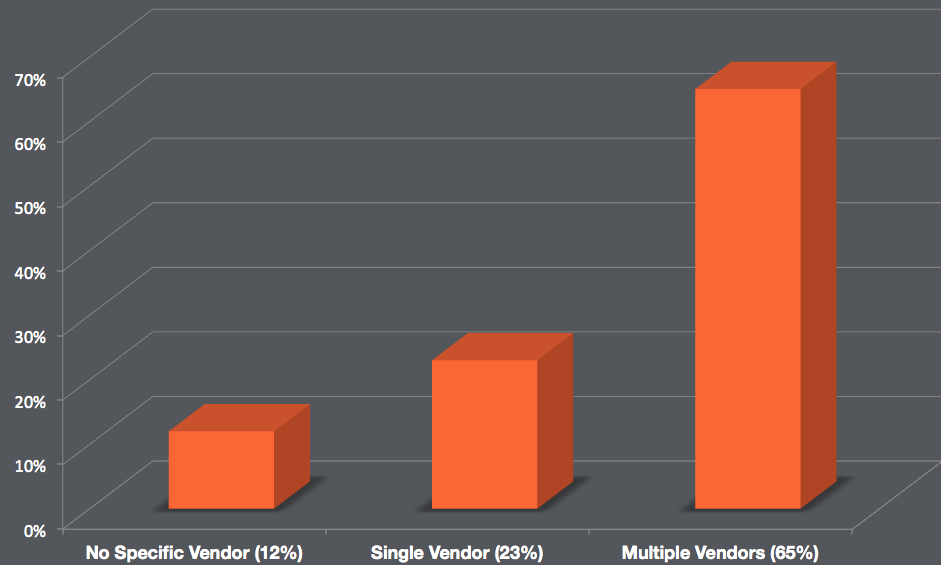
\includegraphics[scale=0.3]{images/graph1.png}
    \end{center}
    \caption{Percentage of companies using multiple vendors}
    \label{fig:graph1}
\end{figure}

According to EMC's report on Global Data Protection Index %[4]
, there exists a direct relationship between the number of vendors that
a company relies on and figures such as IT spending, disruptions, data
loss and the cost of downtime. The more vendors being used, the higher
these damaging numbers climbed. Many companies may feel as if they have
no choice but to use multiple vendors. Often times, backup support is
needed for different operating systems. So, when a company needs support
for both Windows and Linux, they'll often times look to the service of
two vendors; one that supports Windows and one that supports Linux. The
matter of fact is that backup solutions exist that provide support to
more than one operating system. As shown in EMC's report, a single
backup vendor is a financially preferable option for businesses needing
protection over more than one operating system.


\subsubsection{Impact on Disruptions}

Data loss and downtime are a company's worst nightmare. According to
EMC, those organizations using one data protection vendor are the least
likely to experience disruption.

There isn't a significant difference in disruption between companies
using two vendors and those using three or more vendors. However, there
is a significant leap in disruption when compared those using a single
vendor. 54\% of companies using three or more data protection solutions
reported unplanned downtime, while only 42\% of companies using a single
vendor reported downtime. Similarly, 38\% of those using three or more
vendors experienced data loss compared to 24\% of those who use single
vendors.

\subsubsection{Impact on Costs}

Companies who use three or more data protection vendors are being hit
with \$1.66 million in downtime costs. That's more than four times the
amount that it costs those companies who are using just one data
protection vendor (\$0.34 million).


\begin{figure}[t]
    \begin{center}
        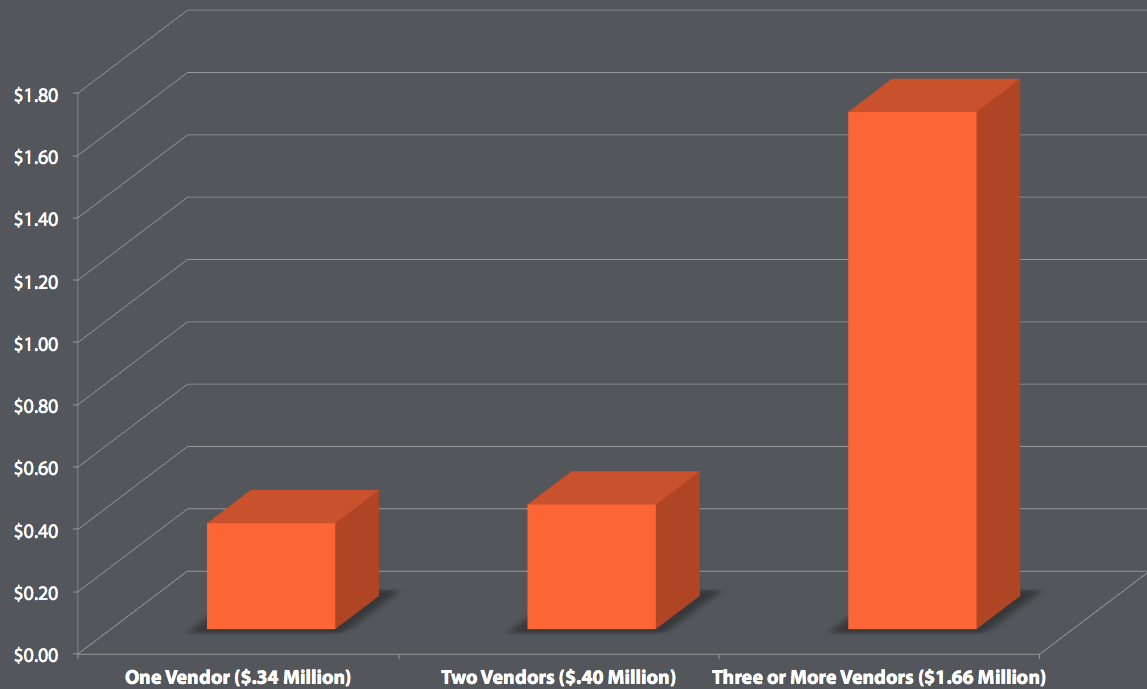
\includegraphics[scale=0.3]{images/graph2.png}
    \end{center}
    \caption{}
    \label{fig:graph2}
\end{figure}

The bottom line is that there is a much greater chance of experiencing
disruption when using multiple data protection vendors, and that using
multiple best-in-breed (highly specialized/cutting edge) solutions can
cause more issues than they claim to solve.


%[4] : http://www.emc.com/collateral/presentation/emc-dpi-key-findings-global.pdf

\section{Future Developments and Requirements}

\subsection{Shift from traditional data structures to ``Big Data''}

As new information is created and handled within the enterprise, IT and
its backup administrators and operators are faced with the challenge of
protecting critical information assets at a much larger scale. Today's
information growth rates have IT organizations at their tipping points.
%[5]
They must ``rethink'' data protection and find the balance between
serving the organization's desire for big data, seeking more value from
the information they create (through data mining and analysis), and the
age old and essential requirement of protecting information from a
disaster, corruption, or a logical or physical system failure.

Meeting the demands of big data backup require both retooling your
approach to data capture and the use of optimization technologies. The
topology of backup targets must evolve from the typical data-centric
model to a more globally dispersed, flexible deployment approach to
achieve better scale and data protection coverage.

\begin{figure}[t]
    \begin{center}
        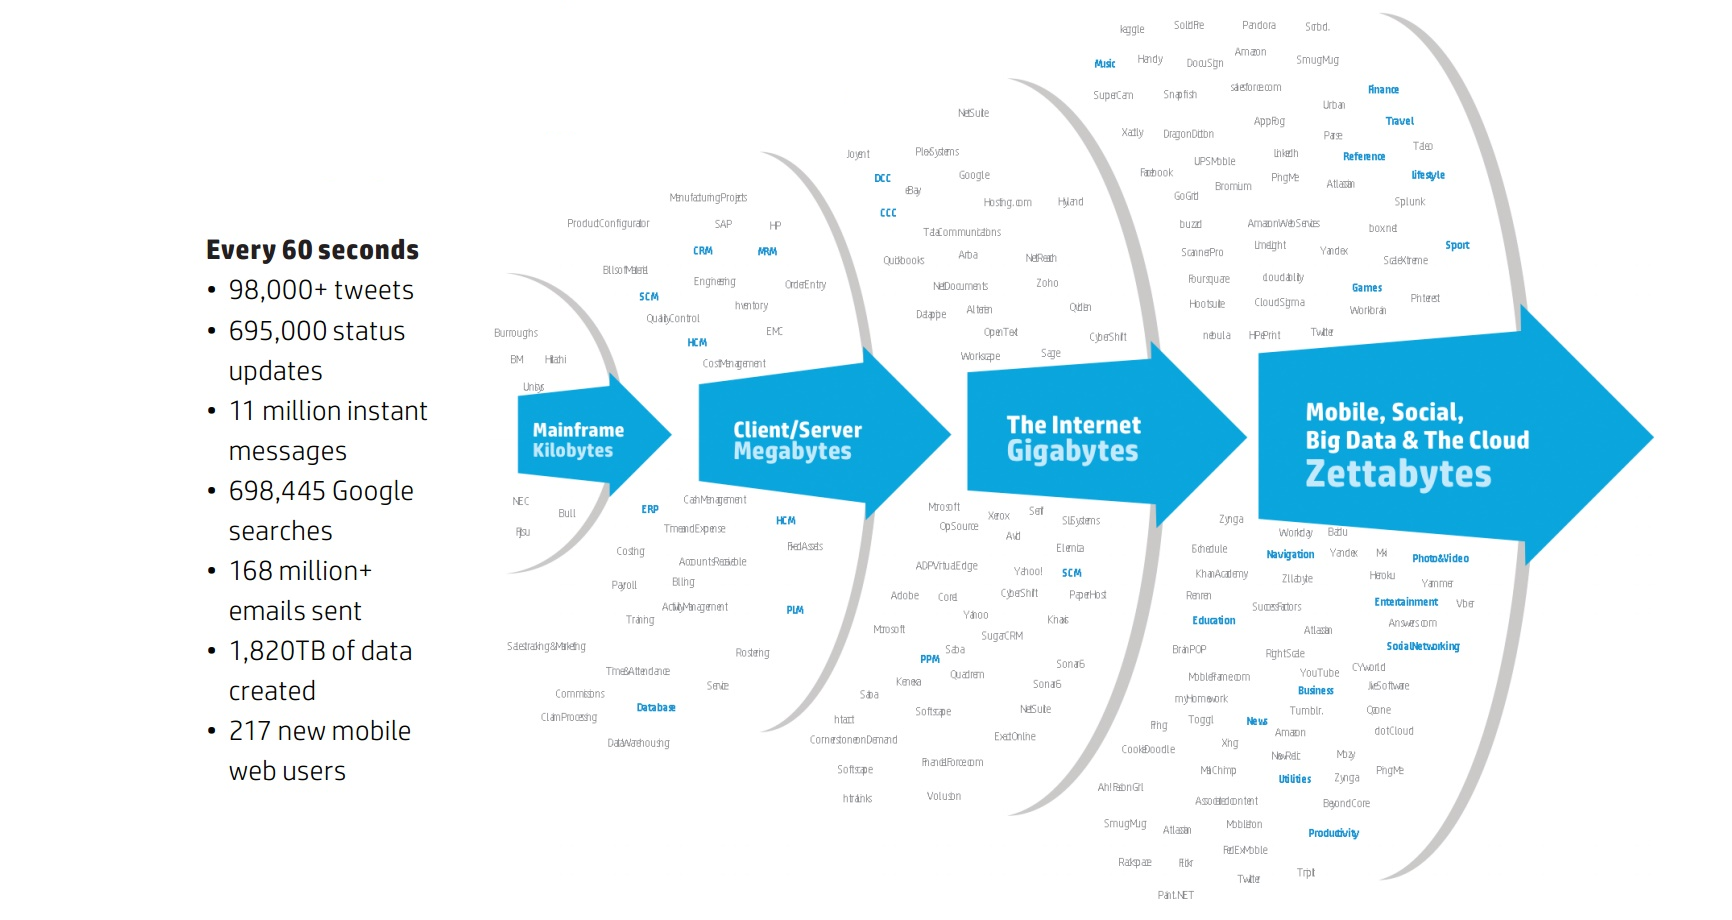
\includegraphics[scale=0.3]{images/graph3.png}
    \end{center}
    \caption{Data volume pace is accelerating}
    \label{fig:graph3}
\end{figure}

Petabyte-size data stores can play havoc with backup windows, and
traditional backup is not designed to handle millions of small files.
Fortunately not all big data information needs to be backed up in the
traditional way. Before considering how to protect your data, you should
decide at what data needs to be protected. Machine-generated data
report data from a database, for instance can be reproduced easier
than it can be backed up and recovered. Compare the cost of protecting
data with the cost of regenerating the data. In many instances, source
data will need to be protected, but any post-acquisition processes may
be cheaper to reproduce than the cost of protecting the data after
manipulation.

Although enterprises have become accustomed to rapid backup data growth,
few are prepared for the avalanche of data that is going to result from
cloud and big data analytics in the coming year and beyond. This data
growth will challenge the capabilities of even the most robust backup
environments. Short-term solutions, solutions with limited scalability,
and solutions that add complexity to the data center will no longer be
viable options.

%[5] : http://esj.com/articles/2012/12/12/big-data-backup-trends.aspx
%[6] : http://h20195.www2.hp.com/V2/GetPDF.aspx/4AA4-6750ENW.pdf

\subsection{Continuous re-evaluation of backup strategy}

Having a clear backup strategy and re-evaluating it according to the
business requirements and needs at least yearly, is necessary to prevent
disaster. The following points need to be addressed and re-evaluated
every time there is a new Business Impact Analysis on backup and
restore.

\begin{itemize}
	\item Address specific business needs. Define a solution for data
		backup as part of a consultative process, while addressing all
		specific business needs.
	\item Conduct TCO analysis. Before moving to a new data backup
		service, a TCO (total cost of ownership) analysis should be done
		to determine the payback period for moving to a new backup
		service. Use a provider that can integrate archives, so you can
		move data sets from a backup plan to an archive plan and
		provides online search and retrieval functionality. And make
		sure your provider has good management processes, good quality
		reporting and a secure facility and connectivity.
	\item Test before provisioning. Put the backup provision in place
		long before you need it.
	\item Encrypt backup data. Security is of prime concern in all forms
		of computing, especially on cloud-based solutions and services.
		To ensure security and privacy always use encrypted backups.
	\item Follow governance and compliance rules. Always make sure to
		follow governance and compliance rules. For example, regulatory
		compliance related to where data may move or be stored when
		different countries or regions are involved, or compliance
		related to retention periods of data. If you are purchasing
		backup service from vendor and a cloud provider then ensure the
		backup service vendor is also following the governing laws for
		that region.
	\item Bulk data import process governance. Data center staff should
		be familiar with process and procedures related to bulk data
		import wherein data is shipped on removable media storage to
		on-premise. This option will be critical when faster data
		recovery is needed for large data backups. In addition customer
		should have in place good governance for data-import process --
		such as who is authorized to receive the removable storage media
		and who is notified.
	\item Backup locally and remotely. Data that is recovered frequently
		should be backed up to both on-premise storage and to cloud
		storage. This is because the on-premise backup assures faster
		recovery, while the off-premise copy can be used for disaster
		recovery purposes.
	\item Backup locally to ensure public accessibility. If the purpose
		of putting data in the cloud is for public accessibility, then
		backup the data locally even before storing in cloud.
	\item Engage multiple vendors. If one can afford it, it is
		recommended to backup very important and critical data to
		multiple vendors to mitigate risks. This gives an extra level of
		safety in case one of the vendors has an outage at a
		business-crucial time.
	\item Ensure data interoperability. Ensure that the backed up data
		can be recovered on premise and/or to another cloud vendor.
\end{itemize}


\subsection{Stress of Uncertainty}

In the end, the stress of uncertainty the last but not least important
factor for the future developments of backup. With key information about
backups divided on multiple, individual systems, IT staff have more
uncertainty to deal with and a harder time making holistic, informed
decisions about their company-wide backup environments.

A solution should be chosen that enables IT data managers to get fast,
accurate information on the status of their entire backup environment.
Robust dashboard functionality can not only enable a single
administrator to manage more backup data, it can also enable them to
reduce inefficiencies in their backup environment, plan for future
capacity needs, and ensure restore Service Level Agreements (SLAs) are
achievable.

While the impact on morale is harder to quantify, the human costs of
sprawl can quickly affect the bottom line with increased staff turnover,
low staff productivity, increased overtime. By consolidating backups and
automating backup tasks, companies can free key IT staff for more
productive and more gratifying work but most importantly achieve their
mission; meeting their SLAs and reducing the business risk of data loss
and downtime.

Scalable, enterprise-class systems also provide a tighter level of
management control and reporting to ensure IT departments get the most
value from their backup investment and more accurate planning for future
needs.


%\section{Review of backup tools and solutions}

%\section{Challenges and potential problems}

%\section{Future developments and requirements}

\nocite{*}
\bibliography{backuprestore}

\end{document}
